\begin{flushright} {\tiny {\color{gray} mms\_dohu03.tex}} \end{flushright}
%~~~~~~~~~~~~~~~~~~~~~~~~~~~~~~~~~~~~~~~~~~~~~~~~~~~~~~~~~~~~~~~~~~~~~~~~~~~~~~~~~~~~~~~~~~~~~~~~~~

Taken from \cite{dohu03}. We consider a two-dimensional problem 
in the square domain $\Omega=[0,1]\times[0,1]$, which possesses a closed-form analytical 
solution. The problem consists of determining the incompressible flow velocity field ${\vec \upnu} = (u,v)$ 
and the pressure $p$ such that 
\begin{eqnarray}
\vec\nabla (2 \eta \dot{\bm \varepsilon}({\vec \upnu})) -{\vec \nabla} p + {\vec b} &=& \vec 0 \quad\quad {\rm in} \; \Omega\\
\vec{\nabla} \cdot \vec{v} &=& 0 \quad\quad {\rm in} \; \Omega\\
\vec{v}&=&\vec{0} \quad\quad {\rm on} \; \Gamma_D
\end{eqnarray}
where the fluid viscosity is taken as $\eta=1$.
The components of the body force $\vec{b}$ are prescribed as 
\begin{eqnarray}
b_x &=& (12 - 24y) x^4 + (-24 + 48y) x^3 + (-48y + 72y^2 - 48 y^3 + 12) x^2 \nonumber\\
    && + (-2 + 24y -72y^2+48y^3)x + 1-4y + 12y^2-8y^3 \nonumber\\ 
b_y &=& (8 - 48y + 48 y^2) x^3 + (-12 + 72y - 72y^2) x^2  \nonumber\\
    && + (4 - 24y + 48y^2 - 48y^3 + 24y^4) x - 12y^2 + 24y^3 - 12y^4  \nonumber
\end{eqnarray}
With this prescribed body force, the exact solution is 
\begin{eqnarray}
u(x,y) &=& x^2(1- x)^2 (2y - 6y^2 + 4y^3) = x^2(1-x)^2 2y (1-3y+2y^2) \nonumber\\
v(x,y) &=& -y^2 (1 - y)^2 (2x - 6x^2 + 4x^3) = -y^2 (1 - y)^2 2x (1-3x+2x^2) \nonumber\\
p(x,y) &=& x(1 -x)- 1/6 \nonumber 
\end{eqnarray}
Note that the pressure obeys $\int_{\Omega} p \; dV = 0$.
One can turn to the spatial derivatives of the fields:
\begin{eqnarray}
\dot{\varepsilon}_{xx}=\frac{\partial u}{\partial x} &=&  (2x -6x^2 +4 x^3 ) (2y - 6y^2 + 4y^3)  \\
\dot{\varepsilon}_{yy}=\frac{\partial v}{\partial y} &=&  - (2x -6x^2 +4 x^3 ) (2y - 6y^2 + 4y^3)  \\
\dot{\varepsilon}_{xy}=\frac{1}{2}\left(\frac{\partial u}{\partial y}+\frac{\partial v}{\partial x}\right) 
&=&=\frac{1}{2}\left( x^2(1- x)^2 ( 2-12y+12y^2  ) -y^2 (1-y)^2 (2-12x+12x^2) \right)
\end{eqnarray}
with of course  ${\vec \nabla} \cdot {\vec \upnu} = 0$ and 
\begin{eqnarray}
\frac{\partial p}{\partial x} &=& 1-2x  \\
\frac{\partial p}{\partial y} &=& 0
\end{eqnarray}

The velocity and pressure fields look like:

\begin{center}
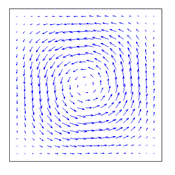
\includegraphics[height=4cm]{images/mms/Ex1_Q2Q1_velo.png}
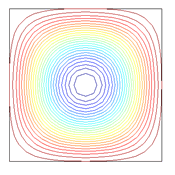
\includegraphics[height=4cm]{images/mms/Ex1_Q2Q1_streamlines.png}
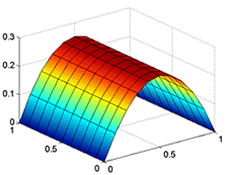
\includegraphics[height=4cm]{images/mms/Ex1_Q2Q1_pres.png}\\
{\small http://ww2.lacan.upc.edu/huerta/exercises/Incompressible/Incompressible\_Ex1.htm}
\end{center}

Then the velocity magnitude is given by 
\begin{eqnarray}
|\vec\upnu|(x,y) 
&=& \sqrt{u^2+v^2} \\
&=& \sqrt{   
[x^2(1-x)^2 2y (1-3y+2y^2)]^2
+ [-y^2 (1 - y)^2 2x (1-3x+2x^2)]^2
} \\
&=& 
\sqrt{   
x^4(1-x)^4 4y^2 (1-3y+2y^2)^2
+ y^4 (1-y)^4 4x^2 (1-3x+2x^2)^2
} \\
&=& 
\sqrt{ 4x^2 y^2} 
\sqrt{   
x^2(1-x)^4 (1-3y+2y^2)^2
+ y^2 (1-y)^4 (1-3x+2x^2)^2
} \\
&=& 
2xy
\sqrt{   
x^2(1-x)^4 (1-3y+2y^2)^2
+ y^2 (1-y)^4 (1-3x+2x^2)^2
} \label{eq:dhvelnorm} 
\end{eqnarray}
This expression is unfortunately not very useful for later postprocessing...

\vspace{.5cm}


As shown in \cite{dohu03}, If the LBB condition is not satisfied, spurious oscillations spoil the pressure approximation. 
Figures below show results obtained with a mesh of 20x20 $Q_1\times P_0$ (left) and $P_1\times P_1$ (right) elements:
\begin{center}
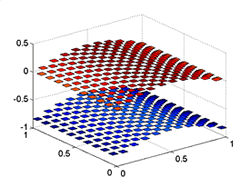
\includegraphics[height=5cm]{images/mms/Ex1_Q1P0_pres.png}
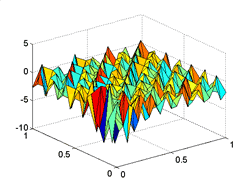
\includegraphics[height=5cm]{images/mms/Ex1_P1P1_pres.png}]]
{\small http://ww2.lacan.upc.edu/huerta/exercises/Incompressible/Incompressible\_Ex1.htm}
\end{center}

Taking into account that the proposed problem has got analytical solution, it is easy to analyze convergence of the different pairs of elements:
\begin{center}
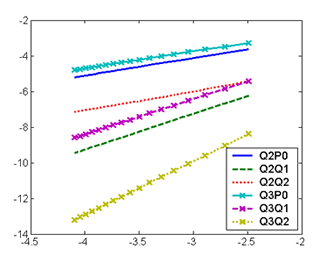
\includegraphics[height=7cm]{images/mms/Ex1_conv_qua.png}\\
{\small http://ww2.lacan.upc.edu/huerta/exercises/Incompressible/Incompressible\_Ex1.htm}
\end{center}

One can also compute the stress components:
\begin{eqnarray}
\sigma_{xx} &=&  2x^2(2x - 2)(4y^3 - 6y^2 + 2y) + 4x(-x + 1)^2*(4y^3 - 6y^2 + 2y) - x(-x + 1) + 1/6 \\
\sigma_{xy} &=&  x^2(-x + 1)^2*(12y^2 - 12y + 2) - y^2(-y + 1)^2*(12x^2 - 12x + 2) \\
\sigma_{yy} &=&  -x(-x + 1) - 2y^2(2y - 2)(4x^3 - 6x^2 + 2x) - 4y(-y + 1)^2(4x^3 - 6x^2 + 2x) + 1/6
\end{eqnarray}

All the necessary functions to do this benchmark are in {\tt mms/dh.py}:
\lstinputlisting[language=python]{mms/dh.py}

This benchmark is implemented in \aspect{} \cite{aspectmanual} and in \stone 1 and many more.

We have
\[
\int_0^1 \int_0^1 u^2 dxdy=
\int_0^1 \int_0^1 ( x^2(1- x)^2 (2y - 6y^2 + 4y^3)  )^2 dx dy = \frac{1}{33075}
\]
\[
\int_0^1 \int_0^1 v^2 dxdy=
\int_0^1 \int_0^1 ( -y^2 (1 - y)^2 (2x - 6x^2 + 4x^3) )^2 dx dy = \frac{1}{33075}
\]
so the root mean square velocity is  
\[
v_{rms} = \sqrt{ \frac{1}{L_x L_y}  \int_0^1 \int_0^1 (u^2+v^2) dx dy } \simeq 0.00777615791
\]

We can also look at depth averages. The vertical depth average of the horizontal component
of the velocity is given by
\begin{eqnarray}
\langle u \rangle (y) 
&=& \frac{1}{L_x} \int_0^{L_x} u(x,y)\; dx \nn\\
&=& \int_0^{L_x} x^2(1-x)^2 2y (1-3y+2y^2) ; dx \nn\\
&=& \left( \int_0^{1} x^2(1-x)^2 \; dx \right) \;   2y (1-3y+2y^2)  \nn\\
&=& \frac{1}{30}2y (1-3y+2y^2) 
\end{eqnarray}
Likewise, the vertical depth average of the vertical component of the velocity is given by
\begin{eqnarray}
\langle v \rangle (y) 
&=& \frac{1}{L_x} \int_0^{L_x} v(x,y)\; dx \nn\\
&=& - \int_0^{1} y^2 (1 - y)^2 2x (1-3x+2x^2)  \; dx \nn\\
&=& - y^2 (1 - y)^2  \left( \int_0^{1}  2x (1-3x+2x^2)  \; dx \right) \nn\\
&=& 0 
\end{eqnarray}

Unfortunately we have seen in Eq.\eqref{eq:dhvelnorm} that the velocity magnitude is 
a rather complex function and we won't be able to compute a depth average analytically.




